\documentclass[journal]{IEEEtran}
\usepackage{amsmath,amssymb}
\usepackage{graphicx}
\usepackage{booktabs}
\usepackage{tabularx}
\usepackage{array}
\usepackage{url}
\usepackage{xurl}
\usepackage{cite}
\usepackage{hyperref}
\hypersetup{hidelinks}
\setlength{\emergencystretch}{3em}
\newcommand{\tightlist}{}

\title{When the Network Twin Drifts: A Candidate-Link Sentinel for Safe OSPF Reconfiguration}
\author{Mohammed Alabdullah%
\thanks{Mohammed Alabdullah is with the Department of Network Engineering,
School of Computer Engineering, Iran University of Science and Technology
(IUST), Tehran, Iran (e-mail:
\href{mailto:m.w@sudo-gate.com}{m.w@sudo-gate.com};
ORCID: \href{https://orcid.org/0009-0001-0826-4380}{0009-0001-0826-4380}).}}

\begin{document}
\maketitle
\begin{abstract}
Network digital twins can validate routing changes before deployment, yet a
control-plane-consistent twin may remain unsafe when operational link performance
has drifted. We study OSPF link-cost reconfiguration in separate
Containerlab/FRRouting operational and twin networks. Both environments
converge to the same candidate route while hidden latency is injected only on
the activated operational link. A false-safe case produces 0.166 ms in the
twin and 66.274 ms operationally against a 50 ms SLA. Static and larger rolling residual margins reject every candidate, while
the only non-vacuous rolling window still admits unsafe changes. We introduce a
candidate-link sentinel that probes the activated link before deployment,
corrects the twin prediction using the operational/twin link discrepancy, and
adds a frozen 0.661 ms margin. Across 186 validation candidates, the policy
accepts 110 changes, admits one unsafe change, and covers 97.32\% of safe
changes. On an untouched 33-sample holdout, it accepts all 19 safe changes and
rejects all 14 unsafe changes. Holdout mean absolute error falls from 40.917
ms to 0.990 ms. Because the upper score covers only 20/33 holdout RTTs, the
result supports empirical safety and utility, not nominal conformal coverage
under distribution shift.
\end{abstract}
\begin{IEEEkeywords}
network digital twin, OSPF, safe network automation, drift, pre-deployment validation, calibrated uncertainty, FRRouting, Containerlab
\end{IEEEkeywords}

\section{Introduction}\label{introduction}

Network digital twins (NDTs) are increasingly proposed as low-risk environments for analyzing network state, evaluating candidate policies, and supporting closed-loop automation. Current architectural work emphasizes that a useful twin is not merely a static topology replica: it depends on data, models, interfaces, and timely information from the physical network {[}1{]}, {[}2{]}. This dependence creates a fundamental operational question. What happens when the control-plane model is correct, but a performance property of the real network has drifted beyond the state represented in the twin?

The question matters for routing changes. Open Shortest Path First (OSPF) derives routes from administratively assigned link costs {[}3{]}, and weight optimization is a long-established traffic-engineering mechanism {[}4{]}. An operator or automation system can therefore evaluate a candidate weight change in a twin and deploy it when the predicted route and performance satisfy policy. However, the candidate can move traffic onto a link whose current latency, loss, or capacity differs from the twin. In that case, agreement on topology, protocol convergence, and next-hop selection does not imply agreement on the service outcome.

Formal configuration-analysis systems can verify broad forwarding and control-plane properties before deployment {[}5{]}, {[}6{]}, {[}7{]}, while consistent-update abstractions protect packet behavior during a configuration transition {[}8{]}. These approaches are essential but address a different failure mode. A configuration may be reachable, loop-free, and installed consistently, yet violate a latency service-level objective because the operational link state is not faithfully represented by the validation model.

This paper studies that gap in a controlled OSPF testbed. We construct separate operational and twin networks using Containerlab and FRRouting. Both networks have the same topology, OSPF configuration, candidate link costs, and resulting routes. We then inject hidden latency drift on the direct link in the operational network only. Lowering the OSPF cost makes both networks select the same direct route, but the twin predicts sub-millisecond latency while the operational path can exceed a 50 ms SLA. This produces a false-safe deployment without a control-plane disagreement.

A first attempt to protect deployment with residual quantiles exposed a second problem. The static margin and rolling windows of 20 and 50 observations rejected every candidate. A rolling window of 10 observations accepted 16 candidates but admitted two unsafe changes and did not retain useful acceptance across all randomized schedules. This result motivates a different observable: before deploying a candidate OSPF change, probe the exact link that the change would activate in both the operational network and the twin. The difference between these link measurements corrects the twin's end-to-end prediction, after which a frozen conformal margin is applied to the deploy/reject decision.

The resulting candidate-link sentinel substantially improves the tested safety--utility trade-off. Across 186 validation changes, the frozen policy accepted 110 candidates, accepted 109 safe candidates, and admitted one unsafe candidate. On an untouched 33-sample holdout, it accepted all 19 safe reconfigurations and rejected all 14 unsafe reconfigurations. The targeted correction reduced mean absolute latency-prediction error from 40.917 ms for the uncorrected twin to 0.990 ms on the holdout. The conformal margin also prevented one unsafe deployment that the raw sentinel would have accepted.

The holdout result must be interpreted carefully. Although the binary deployment decisions were correct for all 33 holdout samples, the nominal 95\% conformal upper-bound coverage did not persist under the shifted residual distribution. The paper therefore makes an empirical claim about the tested latency-drift regime, not a distribution-free safety guarantee. This distinction is consistent with conformal research showing that exchangeability violations require weighted, adaptive, or online treatment {[}9{]}, {[}10{]}, {[}11{]}.

The paper makes four contributions:

\begin{enumerate}
\def\labelenumi{\arabic{enumi}.}
\tightlist
\item
  \textbf{A reproducible false-safe NDT case.} We demonstrate an OSPF reconfiguration for which the operational network and twin agree on the route but disagree on whether the resulting latency satisfies the SLA.
\item
  \textbf{A negative result for residual-only gating.} We show that a global residual-quantile policy can collapse into complete abstention under mixed drift schedules.
\item
  \textbf{A pre-deployment candidate-link sentinel.} We introduce a targeted measurement that is available before deployment and corrects the twin prediction using the link the candidate change would activate.
\item
  \textbf{A separated safety and coverage evaluation.} We report validation and untouched-holdout deployment outcomes while explicitly documenting the failure of nominal conformal predictive coverage under shift.
\end{enumerate}

The present scope is deliberately narrow: one three-router OSPF topology, link-cost changes, and hidden latency drift. This narrow design permits a fully reproducible causal demonstration, but it does not establish behavior under capacity, loss, topology, or multi-link drift, nor at production scale.

\section{Related Work}\label{related-work}

\subsection{Network digital twins}\label{network-digital-twins}

NDT research frames the twin as a virtual representation connected to the physical network through data, models, and interfaces. The current IRTF NMRG reference-architecture draft describes NDTs as a foundation for data-driven management and lower-risk evaluation of network changes {[}1{]}. Complementary data-collection work states that building and updating the twin requires real-time information from the represented network {[}2{]}. These documents are active Internet-Drafts and should be cited as work in progress rather than standards.

Almasan et al.~describe NDT architecture, enabling machine-learning technologies, and a QoS-aware routing-optimization case study {[}12{]}. Hui et al.~organize data-driven network performance modeling around fidelity, efficiency, and flexibility, and identify limited production data as a major challenge {[}13{]}. More recent routing work combines an NDT performance model with what-if route recommendations for transport slicing {[}14{]}. Our work differs by holding control-plane behavior constant and directly testing the risk created by an unobserved performance difference between the twin and the operational network.

Recent systems broaden the operational use of twins. Aether combines agentic AI, verification, simulation, and emulation in an automated change-validation workflow {[}15{]}. MirrorNet reconstructs and synchronizes a production software-defined WAN for high-fidelity emulation {[}16{]}, while REAL reduces the resource cost of running unmodified control-plane containers {[}17{]}. An active architectural draft also integrates NDT capabilities into agent-driven network analysis, decision, validation, and execution {[}18{]}. These works reinforce the importance of accurate and synchronized validation environments. The candidate-link sentinel is narrower: it supplies a quantitative pre-deployment check for the specific link a routing change would activate.

\subsection{OSPF traffic engineering}\label{ospf-traffic-engineering}

OSPF is a link-state interior gateway protocol in which routers compute shortest-path trees from a synchronized topology database and configured metrics {[}3{]}. Fortz and Thorup established OSPF weight optimization as a practical traffic-engineering mechanism and showed that optimized weights can approach general-routing performance in studied networks {[}4{]}. Their problem is selecting effective weights given network and demand information. Our problem begins after a candidate weight change has been selected: whether its predicted performance remains valid when the twin lacks the current latency state of the newly preferred link.

\subsection{Configuration verification and safe updates}\label{configuration-verification-and-safe-updates}

Network configuration analysis can proactively derive forwarding behavior and test properties before deployment. Fogel et al.~combine declarative control-plane modeling with data-plane analysis {[}5{]}. Minesweeper uses symbolic reasoning to verify network-wide properties under modeled environments {[}6{]}, and Plankton combines symbolic partitioning with explicit-state model checking for scalable multi-protocol verification {[}7{]}.

A separate line of work protects the transition between configurations. Reitblatt et al.~define consistent network-update abstractions so packets are processed according to well-defined old or new configurations {[}8{]}. These approaches are complementary to our gate. They can establish route properties and transition correctness, but a performance-SLA failure can remain when the operational link state is outside the model. Our experiments intentionally create this separation: both twin and operational routers install the same OSPF route, while only the operational path experiences hidden latency.

\subsection{Conformal prediction and distribution shift}\label{conformal-prediction-and-distribution-shift}

Conformal prediction offers finite-sample marginal coverage under exchangeability. Tibshirani et al.~extend the framework to covariate shift through importance weighting when the test-to-training density ratio is known or accurately estimated {[}9{]}. Gibbs and Candès propose adaptive conformal inference for online distribution shift {[}10{]} and later develop online inference methods for arbitrary distribution changes {[}11{]}. Bates et al.~provide a related framework for controlling expected prediction-set loss using holdout calibration {[}19{]}.

The present method uses a much simpler frozen split-conformal margin. The margin improved the binary deployment decision in our holdout, but the nominal predictive coverage failed under the shifted residual distribution. We therefore do not claim the guarantees of weighted, adaptive, online, or risk-controlling conformal methods. Instead, these methods define the statistical path for extending the candidate-link sentinel beyond the current controlled experiment.

\subsection{Position relative to prior work}\label{position-relative-to-prior-work}

The reviewed literature separately provides NDT architectures and performance models, OSPF optimization, formal configuration verification, consistent updates, and conformal methods under distribution shift. Our study focuses on their intersection: a candidate OSPF change is control-plane correct and twin-approved, but unsafe because a performance property of the activated link has drifted. The proposed sentinel uses a targeted operational measurement available before deployment, rather than relying exclusively on the global historical residuals of the twin.

\section{System and Threat Model}\label{system-and-threat-model}

\subsection{System scope}\label{system-scope}

We study pre-deployment validation of one class of network changes: modifying OSPF link costs so that traffic is moved from an indirect path to a direct link. The system consists of two isolated but structurally identical environments:

\begin{itemize}
\tightlist
\item
  an \textbf{operational network}, which represents the network in which a candidate change would be deployed; and
\item
  a \textbf{network digital twin}, which is used to simulate the same candidate before deployment.
\end{itemize}

Both environments run unmodified FRRouting 10.5.1 instances inside Containerlab. Each contains three routers, \(r_1,r_2,r_3\), connected as a triangle, and three end hosts, \(h_1,h_2,h_3\), attached to the corresponding routers. IPv4 forwarding is enabled on the router containers, and all router-to-router OSPF interfaces are configured as point-to-point links.

Let the operational and twin topologies be \(G^{o}=(V,E)\) and \(G^{t}=(V,E)\). In the experiment, the node set, link set, IP addressing, OSPF configuration, and candidate configuration are identical between \(G^{o}\) and \(G^{t}\). The environments differ only in an unmodeled performance property injected into the operational network.

\subsection{Baseline and candidate OSPF states}\label{baseline-and-candidate-ospf-states}

The baseline OSPF costs are:

\begin{itemize}
\tightlist
\item
  \(w(r_1,r_2)=10\);
\item
  \(w(r_2,r_3)=10\); and
\item
  \(w(r_1,r_3)=30\).
\end{itemize}

The destination LAN attached to \(r_3\) contributes the default OSPF interface cost of 10. Consequently, the route from \(r_1\) toward \texttt{192.168.13.0/24} has metric 30 through \(r_2\) in the baseline state.

The candidate change \(c\) lowers the OSPF cost of the direct \(r_1\)--\(r_3\) link from 30 to 5 in both directions. After convergence, the destination route has metric 15 and uses the direct next hop at \texttt{192.168.2.2}. The same candidate is evaluated in the operational and twin environments.

\subsection{Service objective and safety label}\label{service-objective-and-safety-label}

The primary service metric is the mean round-trip time from \(h_1\) to \(h_3\), measured using 20 ICMP echo requests. Let

\[
Y^{o}(c)
\]

denote the realized operational mean RTT after candidate \(c\), and let

\[
\widehat{Y}^{t}(c)
\]

denote the mean RTT predicted by executing the candidate in the twin.

The latency service-level threshold is

\[
\tau = 50\text{ ms}.
\]

A realized candidate is labeled safe when

\[
Y^{o}(c) \leq \tau,
\]

and unsafe when

\[
Y^{o}(c) > \tau.
\]

The experiment also records packet loss and the installed route. However, the deployment label used in the present paper is based only on mean RTT. All reported Phase 5 samples retain the same OSPF metric and next hop in the operational network and the twin.

\subsection{Drift model}\label{drift-model}

The drift source is non-malicious performance desynchronization rather than a security attacker. The operational direct link \(r_1\)--\(r_3\) receives an additional \texttt{netem} delay \(d\) on each direction, where

\[
d \in \{0,1,2,5,10,15,20,25,30,35,40\}\text{ ms}.
\]

No corresponding delay is inserted in the twin. Because the impairment is applied in both directions, its RTT contribution is approximately \(2d\), subject to container and scheduling noise.

This construction models a twin that is correct about topology, OSPF state, and the candidate configuration, but stale or incomplete with respect to the current latency of the link that the candidate will activate. It deliberately isolates performance-plane drift from control-plane disagreement.

\subsection{Information available to the deployment policy}\label{information-available-to-the-deployment-policy}

The policy may use the following information before an operational deployment decision:

\begin{enumerate}
\def\labelenumi{\arabic{enumi}.}
\tightlist
\item
  the candidate OSPF change and the link it is expected to activate;
\item
  the candidate's simulated end-to-end RTT in the twin;
\item
  a direct RTT probe of the candidate link in the operational network;
\item
  the corresponding candidate-link probe in the twin;
\item
  the fixed SLA threshold; and
\item
  a margin frozen using an independent calibration set.
\end{enumerate}

The operational post-change RTT \(Y^{o}(c)\) is \textbf{not} a policy input. It is collected only to label the candidate and evaluate the decision.

The experimental harness applies every candidate to the operational network after collecting the pre-deployment probes so that ground-truth outcomes are available for all policies, including candidates that a policy would have rejected. Policy decisions are then replayed from fields available before deployment. A live controller would instead simulate the candidate in the twin, compute the decision, and apply the candidate operationally only when the gate accepts it.

\subsection{Assumptions}\label{assumptions}

The current design makes the following assumptions:

\begin{itemize}
\tightlist
\item
  the candidate link is known from the proposed OSPF change;
\item
  the link remains directly reachable for an active probe before deployment;
\item
  probe traffic is small enough not to materially alter network performance;
\item
  the operational state does not change materially between the probe and the deployment decision;
\item
  the candidate affects one identifiable direct link;
\item
  both OSPF instances converge before end-to-end measurements are collected;
\item
  the latency SLA is known and fixed; and
\item
  calibration observations are not drawn from the final holdout schedule.
\end{itemize}

The implementation identifies the candidate link explicitly for the three-router topology. Automatic candidate-path differencing is a proposed extension, not part of the evaluated artifact.

\subsection{Out-of-scope failures}\label{out-of-scope-failures}

The present threat model does not cover:

\begin{itemize}
\tightlist
\item
  malicious manipulation of probes or telemetry;
\item
  packet-loss, capacity, queueing, or topology drift as the primary impairment;
\item
  simultaneous drift on multiple links;
\item
  failed or unreachable candidate links;
\item
  changes to multiple OSPF weights in one transaction;
\item
  interaction between concurrent controllers;
\item
  transient packet consistency during installation; or
\item
  large-scale and multi-area OSPF networks.
\end{itemize}

These exclusions bound the current claim to empirical latency safety for the tested single-link OSPF reconfiguration.

\section{Candidate-Link Sentinel Method}\label{candidate-link-sentinel-method}

\subsection{Method overview}\label{method-overview}

The candidate-link sentinel augments the twin's simulated end-to-end prediction with a targeted measurement of the link that the candidate OSPF change would activate. The method has four stages:

\begin{enumerate}
\def\labelenumi{\arabic{enumi}.}
\tightlist
\item
  identify the candidate link;
\item
  probe that link in the operational network and the twin;
\item
  correct the twin's candidate prediction using the observed link mismatch;
\item
  add a one-sided calibration margin and compare the result with the SLA.
\end{enumerate}

The targeted probe is available even when the candidate is ultimately rejected. This differs from residual-only adaptation, which may depend on observing post-deployment outcomes.

\subsection{Candidate-link measurement}\label{candidate-link-measurement}

For candidate \(c\), let \(e_c\) be the link expected to become preferred after the OSPF cost change. The current implementation fixes

\[
e_c = (r_1,r_3).
\]

Before changing the operational OSPF cost, \(r_1\) sends 20 ICMP echo requests to the directly connected \(r_3\) address \texttt{192.168.2.2}. Addressing the neighbor interface directly forces the probe over \(e_c\), even while the baseline route toward \(h_3\) still traverses \(r_2\).

Let

\[
L^{o}(e_c)
\]

be the operational mean candidate-link RTT, and let

\[
L^{t}(e_c)
\]

be the corresponding mean RTT in the twin.

The measured one-sided link discrepancy is

\[
\Delta(c) =
\max\left(0,\;L^{o}(e_c)-L^{t}(e_c)\right).
\]

The maximum with zero makes the correction conservative for an upper-latency SLA: an operational link that is faster than its twin does not reduce the predicted RTT, while a slower operational link increases it.

\subsection{Corrected candidate prediction}\label{corrected-candidate-prediction}

The candidate is simulated in the twin to obtain the end-to-end prediction

\[
\widehat{Y}^{t}(c).
\]

The sentinel-corrected prediction is

\[
\widetilde{Y}(c)
=
\widehat{Y}^{t}(c)+\Delta(c).
\]

This correction assumes that the dominant operational/twin discrepancy lies on the newly activated link and that the link-level RTT difference transfers approximately to the end-to-end path. The assumption is appropriate for the controlled single-link latency experiment, but it is not a general decomposition theorem.

\subsection{Calibration residual}\label{calibration-residual}

For calibration candidate \(i\), the signed one-sided residual is

\[
R_i =
Y^{o}_i-\widetilde{Y}_i.
\]

Positive residuals indicate that the realized operational RTT exceeded the corrected prediction. Because the objective is an upper latency bound, the method uses an upper residual quantile rather than the absolute residual.

Let \(n\) be the number of independent calibration observations and \(\alpha\) the target tail level. The finite-sample order-statistic rank is

\[
k =
\min\left(
n,\;
\left\lceil(n+1)(1-\alpha)\right\rceil
\right).
\]

After sorting the residuals as \(R_{(1)}\leq\cdots\leq R_{(n)}\), the margin is

\[
q_{\alpha}=R_{(k)}.
\]

For the frozen policy,

\[
n=22,\qquad
\alpha=0.05,\qquad
k=22,\qquad
q_{\alpha}=0.661\text{ ms}.
\]

The margin is computed once from \texttt{calibration\_seed77} and is not updated using validation or holdout outcomes.

\subsection{Deployment rule}\label{deployment-rule}

The one-sided upper score for candidate \(c\) is

\[
U(c)=\widetilde{Y}(c)+q_{\alpha}.
\]

The frozen deployment policy is

\[
\pi(c)=
\begin{cases}
1, & U(c)\leq\tau,\\
0, & U(c)>\tau,
\end{cases}
\]

where \(\pi(c)=1\) means deploy and \(\pi(c)=0\) means reject.

For the present experiment, \(\tau=50\) ms and \(q_{\alpha}=0.661\) ms. No policy parameter is changed after the validation decision is frozen.

\subsection{Policy pseudocode}\label{policy-pseudocode}

\begin{verbatim}
Input:
    candidate c
    candidate link e_c
    SLA threshold tau
    frozen residual margin q_alpha

1. Simulate c in the network twin.
2. Measure twin candidate RTT: y_twin.
3. Probe e_c operationally.
   Store the result as l_ops.
4. Probe e_c in the twin: l_twin.
5. delta <- max(0, l_ops - l_twin)
6. corrected <- y_twin + delta
7. upper <- corrected + q_alpha
8. if upper <= tau:
       return DEPLOY
   else:
       return REJECT
\end{verbatim}

In the experimental harness, Step 1 is followed by applying the candidate to the operational network solely to collect \(Y^{o}(c)\) for evaluation. That ground-truth measurement is not used in Steps 3--8.

Although Phases 4 and 5 share schedule definitions, their measurements were collected independently. Consequently, threshold-near observations differ: Phase 4 contains 121 safe and 65 unsafe validation outcomes, whereas Phase 5 contains 112 safe and 74 unsafe outcomes.

\subsection{Compared policies}\label{compared-policies}

The experiment evaluates four deployment policies:

\subsubsection{Direct deployment}\label{direct-deployment}

\[
\pi_{\text{direct}}(c)=1.
\]

Every candidate is deployed without twin validation.

\subsubsection{Twin-only validation}\label{twin-only-validation}

\[
\pi_{\text{twin}}(c)
=
\mathbb{1}
\left[
\widehat{Y}^{t}(c)\leq\tau
\right].
\]

This policy trusts the uncorrected twin prediction.

\subsubsection{Raw candidate-link sentinel}\label{raw-candidate-link-sentinel}

\[
\pi_{\text{raw}}(c)
=
\mathbb{1}
\left[
\widetilde{Y}(c)\leq\tau
\right].
\]

This policy uses the candidate-link correction without a residual margin.

\subsubsection{Conformal candidate-link sentinel}\label{conformal-candidate-link-sentinel}

\[
\pi_{\text{sentinel}}(c)
=
\mathbb{1}
\left[
\widetilde{Y}(c)+q_{\alpha}\leq\tau
\right].
\]

This is the policy frozen before holdout evaluation.

\subsection{Validation-selection rule}\label{validation-selection-rule}

A candidate policy is considered operationally non-vacuous only when it accepts at least one candidate and at least one safe candidate. It must also accept a safe candidate in every validation schedule. Among policies satisfying these conditions, selection minimizes the number of unsafe deployments, then maximizes safe-change coverage, then maximizes total acceptance.

This rule prevents a policy from being selected merely because it rejects every candidate. In Phase 4, residual-only rolling policies with windows 20 and 50 had zero unsafe deployments but also zero accepted candidates; they were therefore rejected as vacuous.

\subsection{Evaluation metrics}\label{evaluation-metrics}

For \(N\) candidates, let \(D_i=\pi(c_i)\) be the binary deployment decision and let

\[
Z_i=\mathbb{1}[Y^{o}_i>\tau]
\]

be the unsafe label.

The acceptance rate is

\[
\mathrm{AR}
=
\frac{1}{N}\sum_{i=1}^{N}D_i.
\]

The number of unsafe deployments is

\[
\mathrm{UD}
=
\sum_{i=1}^{N}D_iZ_i.
\]

The unsafe rate among accepted candidates is

\[
\mathrm{URA}
=
\frac{\sum_i D_iZ_i}
     {\sum_i D_i},
\]

when at least one candidate is accepted.

Safe-change coverage is

\[
\mathrm{SC}
=
\frac{
\sum_i D_i(1-Z_i)
}{
\sum_i (1-Z_i)
}.
\]

The paper also reports mean absolute prediction error, root mean squared prediction error, route agreement, and Wilson confidence intervals for binomial rates.

\subsection{Computational cost}\label{computational-cost}

For a fixed candidate link and \(P\) probe packets, the online arithmetic is constant time after measurement. The measurement cost is \(O(P)\), while twin simulation and OSPF convergence dominate wall-clock latency. Calibration requires sorting \(n\) residuals, with \(O(n\log n)\) time and \(O(n)\) storage. The current artifact does not measure controller runtime overhead separately.

\subsection{Statistical interpretation}\label{statistical-interpretation}

The margin is split-conformal-style, but the paper does not claim that it retains nominal 95\% predictive coverage under arbitrary drift. On the untouched holdout, the binary deployment classifier separated all tested safe and unsafe candidates, while the upper score covered only 20 of 33 realized RTTs. The supported conclusion is therefore empirical evidence of safety and utility in the tested latency-drift regime, not a distribution-free coverage or zero-risk guarantee.

\section{Experimental Methodology}\label{experimental-methodology}

\subsection{Research questions}\label{research-questions}

The evaluation addresses four research questions:

\begin{itemize}
\tightlist
\item
  \textbf{RQ1 --- False-safe twin behavior:} Can an OSPF candidate be control-plane consistent between the operational network and its twin while violating the operational latency SLA?
\item
  \textbf{RQ2 --- Residual-only gating:} Does a global residual-calibration policy retain useful acceptance under heterogeneous and shifted delay schedules?
\item
  \textbf{RQ3 --- Targeted drift sensing:} Does probing the candidate link before deployment improve latency prediction and the safety--utility trade-off?
\item
  \textbf{RQ4 --- Untouched evaluation after freezing:} Does the selected policy retain useful behavior on a randomized holdout that is not used for calibration or policy selection?
\end{itemize}

The experiment is designed as a controlled causal study rather than a production-scale benchmark. The manipulated variable is the hidden per-direction latency on the operational candidate link; the twin topology, routing configuration, candidate configuration, and host workloads are held constant.

\subsection{Execution environment}\label{execution-environment}

Experiments run on an Apple-silicon MacBook Pro using an Ubuntu machine provided by OrbStack. Containerlab version 0.77.0 orchestrates the network containers.

Routers use:

\begin{verbatim}
quay.io/frrouting/frr:10.5.1
\end{verbatim}

End hosts use:

\begin{verbatim}
wbitt/network-multitool:3.22.2
\end{verbatim}

The operational laboratory is named \texttt{ospf-ops}, and the twin laboratory is named \texttt{ospf-twin}. Each environment runs independently so that operational impairments do not modify the twin.

\subsection{Network topology}\label{network-topology}

Each environment contains three FRRouting routers arranged in a triangle,
with one host attached to each router.

\begin{figure}[t]
\centering
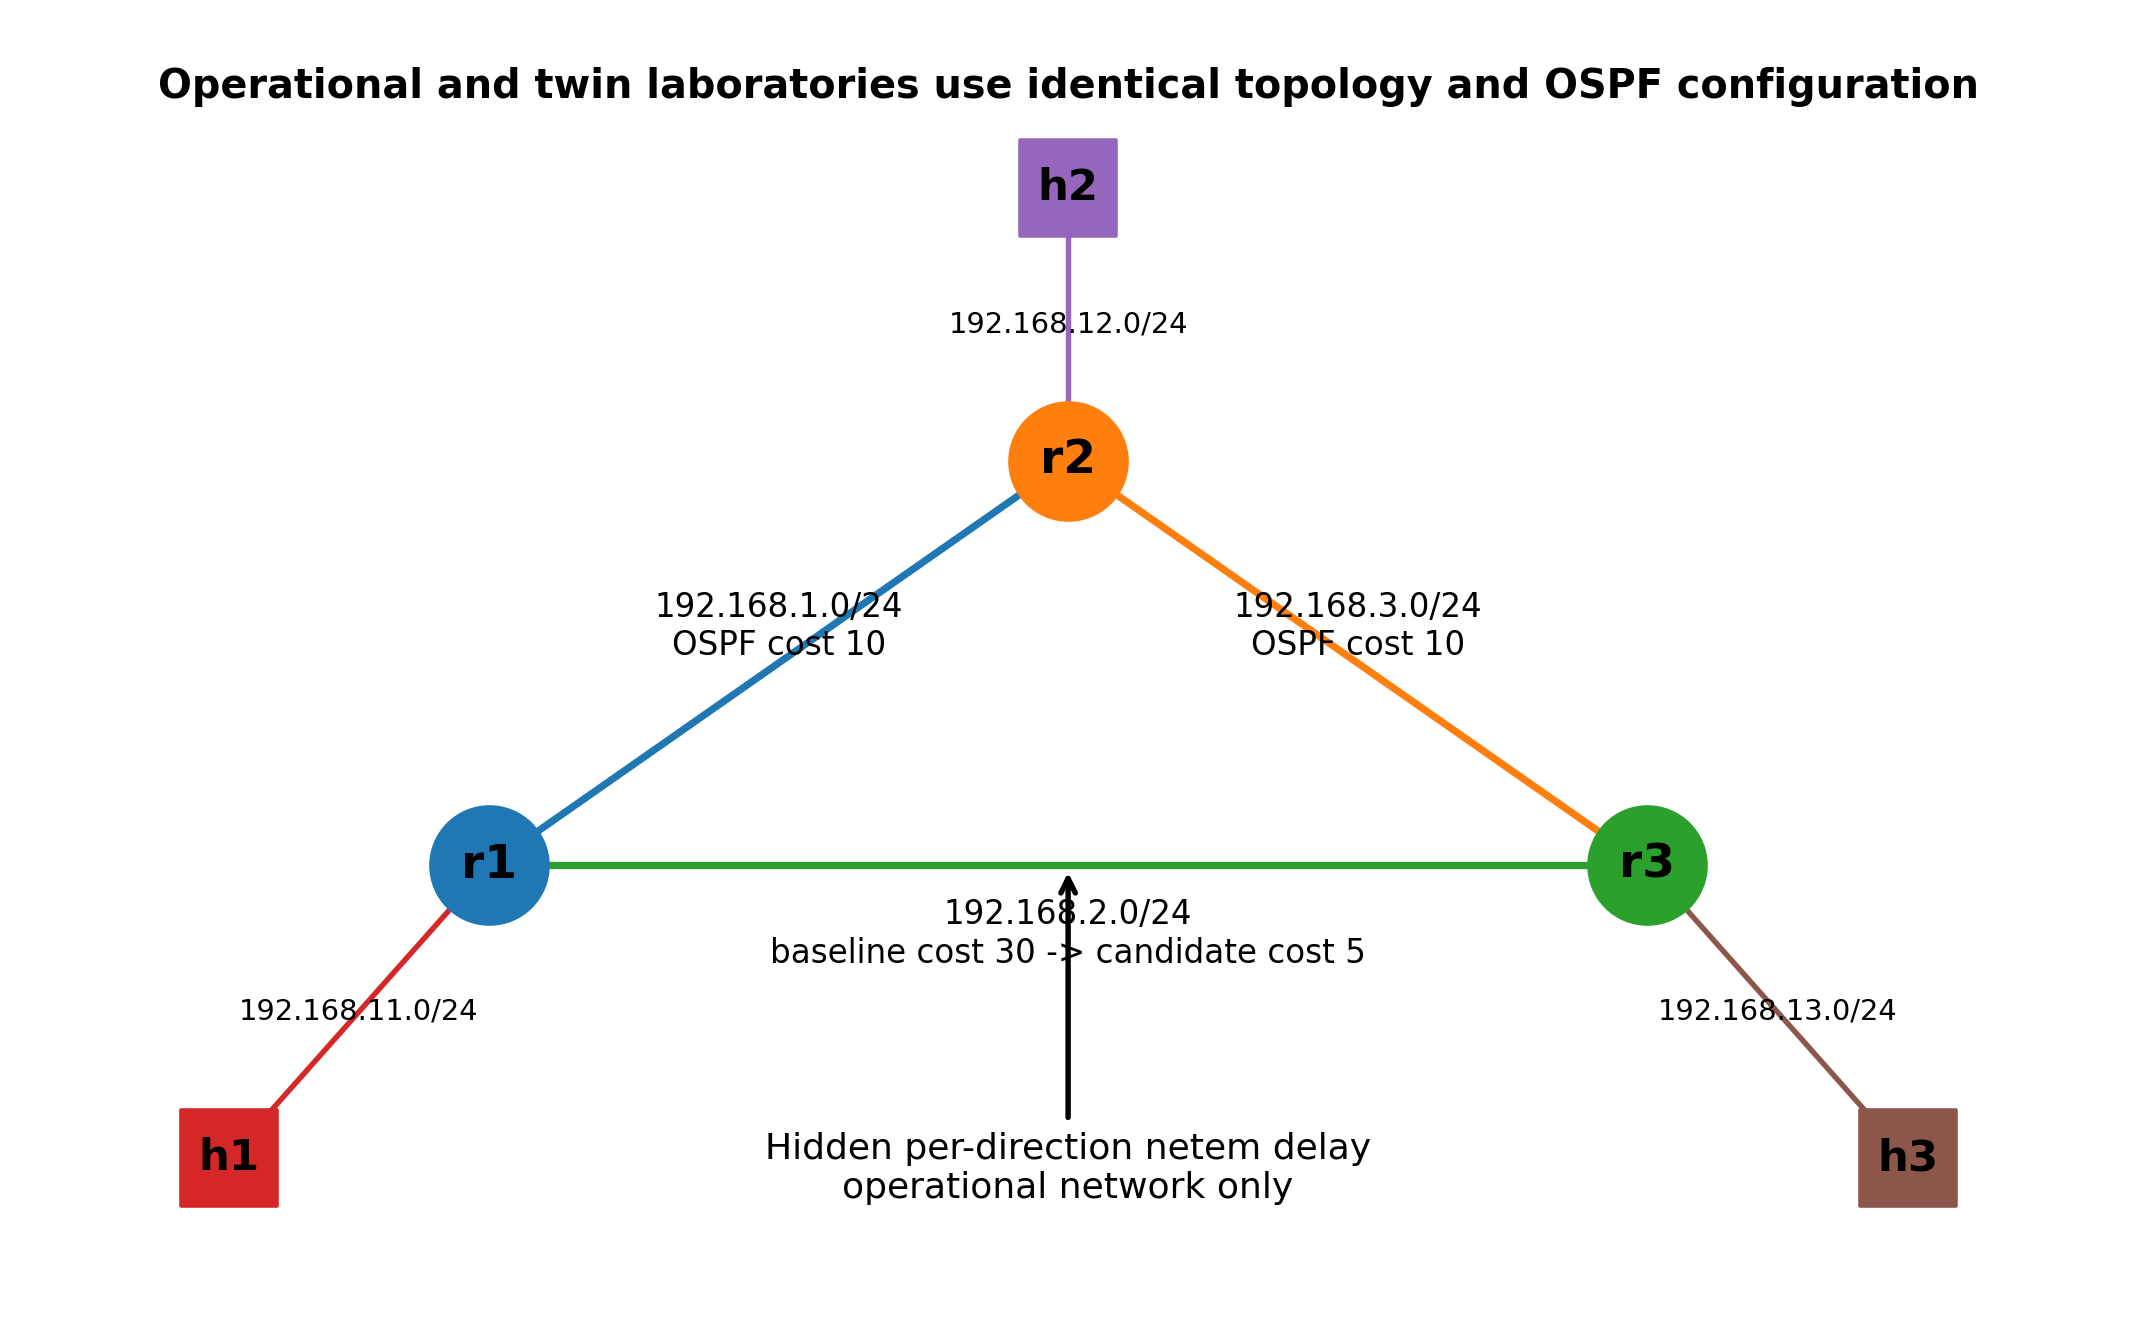
\includegraphics[width=\columnwidth]{figures/figure0_testbed_topology.png}
\caption{Experimental topology shared by the operational and twin
laboratories. Hidden \texttt{netem} delay is applied only to the operational
\(r_1\)--\(r_3\) candidate link.}
\label{fig:testbed-topology}
\end{figure}

The number on each router-to-router edge denotes the baseline OSPF cost. Host \(h_2\) is attached to \(r_2\), although the primary measured flow is \(h_1\rightarrow h_3\).

The candidate changes the direct \(r_1\)--\(r_3\) cost from 30 to 5 on both ends. The baseline route from \(r_1\) to the LAN behind \(r_3\) uses \(r_2\) and has metric 30. The candidate route uses the direct link and has metric 15, including the destination-interface cost.

Before each schedule, a readiness script confirms:

\begin{enumerate}
\def\labelenumi{\arabic{enumi}.}
\tightlist
\item
  both laboratories are deployed;
\item
  every expected OSPF adjacency is in the \texttt{Full/-} state;
\item
  the destination route is installed; and
\item
  \(h_1\) can reach \(h_3\).
\end{enumerate}

\subsection{Controlled drift injection}\label{controlled-drift-injection}

The operational candidate link is the direct \(r_1\)--\(r_3\) connection. The experiment applies Linux \texttt{netem} delay to the corresponding interface on both operational endpoints. The twin receives no delay modification.

The per-direction delay levels are

\[
D =
\{0,1,2,5,10,15,20,25,30,35,40\}
\text{ ms}.
\]

Applying delay in both directions produces an approximate round-trip contribution of \(2d\), with normal container and host-scheduling variation.

For each sample, the harness first sets the requested delay and returns OSPF to the baseline cost state. After the sample has been parsed, the next sample sets its own delay and baseline state. At the end of a schedule, delay is reset to zero and the baseline costs are restored.

\subsection{Per-sample protocol}\label{per-sample-protocol}

Each sample executes the following sequence:

\begin{enumerate}
\def\labelenumi{\arabic{enumi}.}
\tightlist
\item
  apply the operational delay level;
\item
  set operational and twin OSPF costs to the baseline state;
\item
  send 20 ICMP probes from operational \(r_1\) to operational \texttt{192.168.2.2};
\item
  send the corresponding 20 probes in the twin;
\item
  set both environments to the candidate OSPF state;
\item
  record the installed route to \texttt{192.168.13.0/24} in both environments;
\item
  send 20 end-to-end ICMP probes from \(h_1\) to \(h_3\) in each environment; and
\item
  parse the measurements into a structured sample summary.
\end{enumerate}

Pings use an interval of 0.1 s and a response timeout of 2 s. The parser records packet-loss percentage and minimum, mean, maximum, and variation of RTT. FRRouting's BusyBox-style three-value link-probe summary is supported by treating the missing variation field as zero.

The scripts do not override ICMP payload size, so each container's default \texttt{ping} payload is used. No warm-up request or first reply is discarded: the reported mean is the summary mean over all received replies from the 20 requests. The candidate-state script waits 2 s after updating the OSPF cost on both endpoints before route and end-to-end measurements are collected.

The direct link probes occur before the operational candidate is applied. The post-change operational end-to-end measurement is collected only to construct ground truth for evaluation. It is not an input to the deploy/reject rule.

\subsection{Dataset partitions}\label{dataset-partitions}

\subsubsection{Calibration}\label{calibration}

The calibration schedule \texttt{calibration\_seed77} contains 22 samples: two observations for each of the 11 delay levels. Their order is randomized using seed 77. These samples determine the fixed one-sided residual margin.

\subsubsection{Validation}\label{validation}

Policy selection uses 186 validation samples from five schedules:

\begin{table*}[t]
\caption{Validation schedules and their experimental purpose.}
\centering
\scriptsize
\begin{tabularx}{\textwidth}{XXX}
\toprule
Schedule & Samples & Design purpose \\
\midrule
\texttt{randomized\_seed101} & 33 & Three randomized repetitions of each delay \\
\texttt{randomized\_seed202} & 33 & Independent randomized ordering \\
\texttt{randomized\_seed303} & 33 & Independent randomized ordering \\
\texttt{abrupt\_shift} & 45 & Low-delay regime, abrupt high-delay regime, then recovery \\
\texttt{up\_down} & 42 & Repeated ascending and descending delay sweeps \\
**Total** & **186** &  \\
\bottomrule
\end{tabularx}
\end{table*}

The three randomized schedules expose the policy to order variation while preserving the same delay support. The abrupt-shift and up/down schedules test whether policy utility depends on a stationary or smoothly ordered sequence.

\subsubsection{Untouched holdout}\label{untouched-holdout}

The holdout schedule \texttt{holdout\_seed909} contains 33 samples: three observations for each of the 11 delay levels in a randomized order generated with seed 909.

The holdout is not used to compute the margin, compare candidate policies, or select a policy. The policy manifest fixes the method, SLA, calibration size, order-statistic rank, residual margin, prediction rule, and deployment rule before holdout evaluation.

\subsection{Experimental phases}\label{experimental-phases}

The artifact records the development process as separate phases.

\subsubsection{Phase 1 --- convergence smoke test}\label{phase-1-convergence-smoke-test}

The first phase verifies that the three-router OSPF laboratory converges and that changing the direct-link cost moves traffic to the intended route.

\subsubsection{Phase 2 --- first false-safe twin case}\label{phase-2-first-false-safe-twin-case}

A hidden 30 ms per-direction delay is applied to the operational direct link. After the candidate OSPF change, both environments select the direct route. The twin predicts a sub-millisecond RTT, whereas the operational RTT is about 66 ms and violates the 50 ms SLA. This establishes RQ1.

\subsubsection{Phase 3 --- delay sweep and preliminary gates}\label{phase-3-delay-sweep-and-preliminary-gates}

A 55-sample delay sweep explores the relation between injected delay, operational RTT, twin error, and residual-based gates. This phase is exploratory and is not used as the final untouched holdout.

\subsubsection{Phase 4 --- residual-only policy validity}\label{phase-4-residual-only-policy-validity}

A 22-sample calibration set and 186 validation samples evaluate static and rolling residual policies. The static policy and rolling windows of 20 and 50 observations reject every candidate. The rolling window of 10 observations is non-vacuous but admits two unsafe changes and fails the cross-schedule utility criterion. These results motivate method revision.

\subsubsection{Phase 5 --- candidate-link sentinel}\label{phase-5-candidate-link-sentinel}

The candidate-link sentinel uses the same schedule definitions and the same 22/186 calibration-validation sizes, but Phase 5 is an independent measurement run rather than a reuse of Phase 4 records. The calibrated sentinel is selected and frozen before the 33-sample holdout is evaluated once.

\subsection{Compared policies}\label{compared-policies-1}

Four policies are evaluated from the same sample records:

\begin{itemize}
\tightlist
\item
  \textbf{Direct:} deploy every candidate.
\item
  \textbf{Twin only:} deploy when twin end-to-end RTT is at most 50 ms.
\item
  \textbf{Raw sentinel:} deploy when the corrected prediction is at most 50 ms.
\item
  \textbf{Conformal sentinel:} deploy when the corrected prediction plus the frozen 0.661 ms margin is at most 50 ms.
\end{itemize}

Using common sample records permits paired comparison. Every policy receives the same pre-deployment observables and ground-truth label.

\subsection{Policy-selection protocol}\label{policy-selection-protocol}

Candidate policies are compared only on calibration and validation data. A policy is ineligible when it:

\begin{itemize}
\tightlist
\item
  accepts no candidates;
\item
  accepts no safe candidate; or
\item
  fails to accept at least one safe candidate in every validation schedule.
\end{itemize}

Among eligible policies, selection is lexicographic:

\begin{enumerate}
\def\labelenumi{\arabic{enumi}.}
\tightlist
\item
  minimize unsafe deployments;
\item
  maximize safe-change coverage; and
\item
  maximize total acceptance.
\end{enumerate}

This protocol explicitly rejects complete abstention as a misleading safety result.

The selected conformal candidate-link sentinel is recorded in \texttt{frozen\_policy.json} with:

\begin{itemize}
\tightlist
\item
  calibration size 22;
\item
  \(\alpha=0.05\);
\item
  finite-sample rank 22;
\item
  margin 0.661 ms;
\item
  latency SLA 50 ms;
\item
  the exact prediction and deployment rules; and
\item
  SHA-256 hashes of the validation inputs.
\end{itemize}

\subsection{Holdout execution and incident disclosure}\label{holdout-execution-and-incident-disclosure}

The holdout runner checks that the frozen-policy manifest exists and that no completed holdout-results file is present. It refuses a second evaluation after \texttt{holdout\_results.json} has been created.

During the first holdout sample, raw measurements were collected before the policy manifest had been committed because the results directory was ignored by the initial \texttt{.gitignore}. Parsing then stopped because the link probe used a three-value BusyBox ping summary rather than the four-value format expected by the parser.

The raw first-sample files were preserved. The parser was modified only to accept both ping formats, and the existing measurements were parsed without remeasurement. No margin, SLA, policy rule, schedule, or sample value was changed. The policy file and parser correction were committed in a new commit, and the holdout runner skipped the completed first summary before collecting the remaining 32 samples. The incident is disclosed in \path{docs/holdout_execution_log.md}.

This sequence means the first measurement preceded the Git commit containing the manifest, although the policy parameters already existed in the file and were not modified after measurement. The paper should describe the holdout as untouched for policy selection while transparently reporting this procedural deviation.

\subsection{Outcome variables}\label{outcome-variables}

The primary policy outcomes are:

\begin{itemize}
\tightlist
\item
  accepted candidates;
\item
  unsafe deployments;
\item
  unsafe rate among accepted candidates;
\item
  safe accepted candidates;
\item
  safe rejected candidates;
\item
  safe-change coverage; and
\item
  acceptance rate.
\end{itemize}

Prediction quality is reported using:

\begin{itemize}
\tightlist
\item
  mean absolute error;
\item
  root mean squared error;
\item
  corrected residuals; and
\item
  Pearson correlation between corrected prediction and observed RTT.
\end{itemize}

The experiment also checks route agreement between the operational network and twin.

\subsection{Statistical reporting}\label{statistical-reporting}

For proportions, the analysis reports 95\% Wilson confidence intervals. A zero observed unsafe count is not reported as proof of zero true risk.

The conformal upper score is separately evaluated as a predictive bound. This distinguishes:

\begin{enumerate}
\def\labelenumi{\arabic{enumi}.}
\tightlist
\item
  binary deployment-classification performance relative to the 50 ms SLA; and
\item
  empirical coverage of realized RTT by the upper score.
\end{enumerate}

This distinction is necessary because the holdout decisions were all correct, while the nominal 95\% upper-bound coverage was not achieved.

\subsection{Integrity and reproducibility controls}\label{integrity-and-reproducibility-controls}

The artifact uses the following controls:

\begin{itemize}
\tightlist
\item
  generated schedules are stored as CSV files;
\item
  processed rows preserve sample ID, schedule, position, delay, repetition, role, and seed;
\item
  validation and holdout results are stored as JSON;
\item
  the policy manifest records source hashes;
\item
  holdout-result files prevent automatic second execution;
\item
  dated provenance records separate policy freezing, holdout completion, evaluator correction, and final analysis;
\item
  analysis files record the parser incident and evaluator correction; and
\item
  the final holdout dataset is checked for 33 unique IDs, positions 1--33, three repetitions per delay, consistent safety labels, and universal route agreement.
\end{itemize}

\subsection{Threats to validity}\label{threats-to-validity}

\subsubsection{Internal validity}\label{internal-validity}

Container scheduling and active-probe variation introduce measurement noise. The use of 20 probes per measurement reduces but does not eliminate this variation. All policies are evaluated on the same samples, limiting between-policy confounding.

The experimental harness applies rejected candidates to collect their counterfactual operational outcomes. This differs from live enforcement but is necessary to estimate false-safe and false-reject decisions. The policy logic is computed only from information available before deployment.

\subsubsection{Construct validity}\label{construct-validity}

Mean ICMP RTT is a narrow proxy for service performance. The experiment does not establish behavior for application latency, tail latency, throughput, packet loss, or congestion.

\subsubsection{External validity}\label{external-validity}

The topology contains three routers, one OSPF area, one candidate link, and a single weight change. Results cannot be assumed to generalize to large, multi-area, multi-vendor, or highly dynamic production networks.

\subsubsection{Statistical conclusion validity}\label{statistical-conclusion-validity}

The calibration and holdout sets are small. Confidence intervals remain wide, and the nominal conformal coverage assumption is violated under the observed residual shift. The main conclusion is therefore an empirical demonstration and not a universal risk guarantee.

\section{Results}\label{results}

\subsection{RQ1: A route-consistent twin can make a false-safe latency decision}\label{rq1-a-route-consistent-twin-can-make-a-false-safe-latency-decision}

The baseline and hidden-drift experiment isolates performance-plane desynchronization. Before drift, the operational network and twin use the indirect route through \(r_2\), both with OSPF metric 30. Their mean end-to-end RTTs are 0.153 ms and 0.184 ms, respectively.

After a 30 ms per-direction delay is hidden on the operational direct link, the candidate OSPF change causes both environments to select next hop \texttt{192.168.2.2} with metric 15. The twin reports 0.166 ms and therefore predicts that the candidate satisfies the 50 ms SLA. The operational network instead measures 66.274 ms, producing a 66.108 ms residual and violating the SLA.

This is a false-safe decision without route disagreement: the modeled control-plane outcome is correct, but the modeled performance state is not.

\begin{figure}
\centering
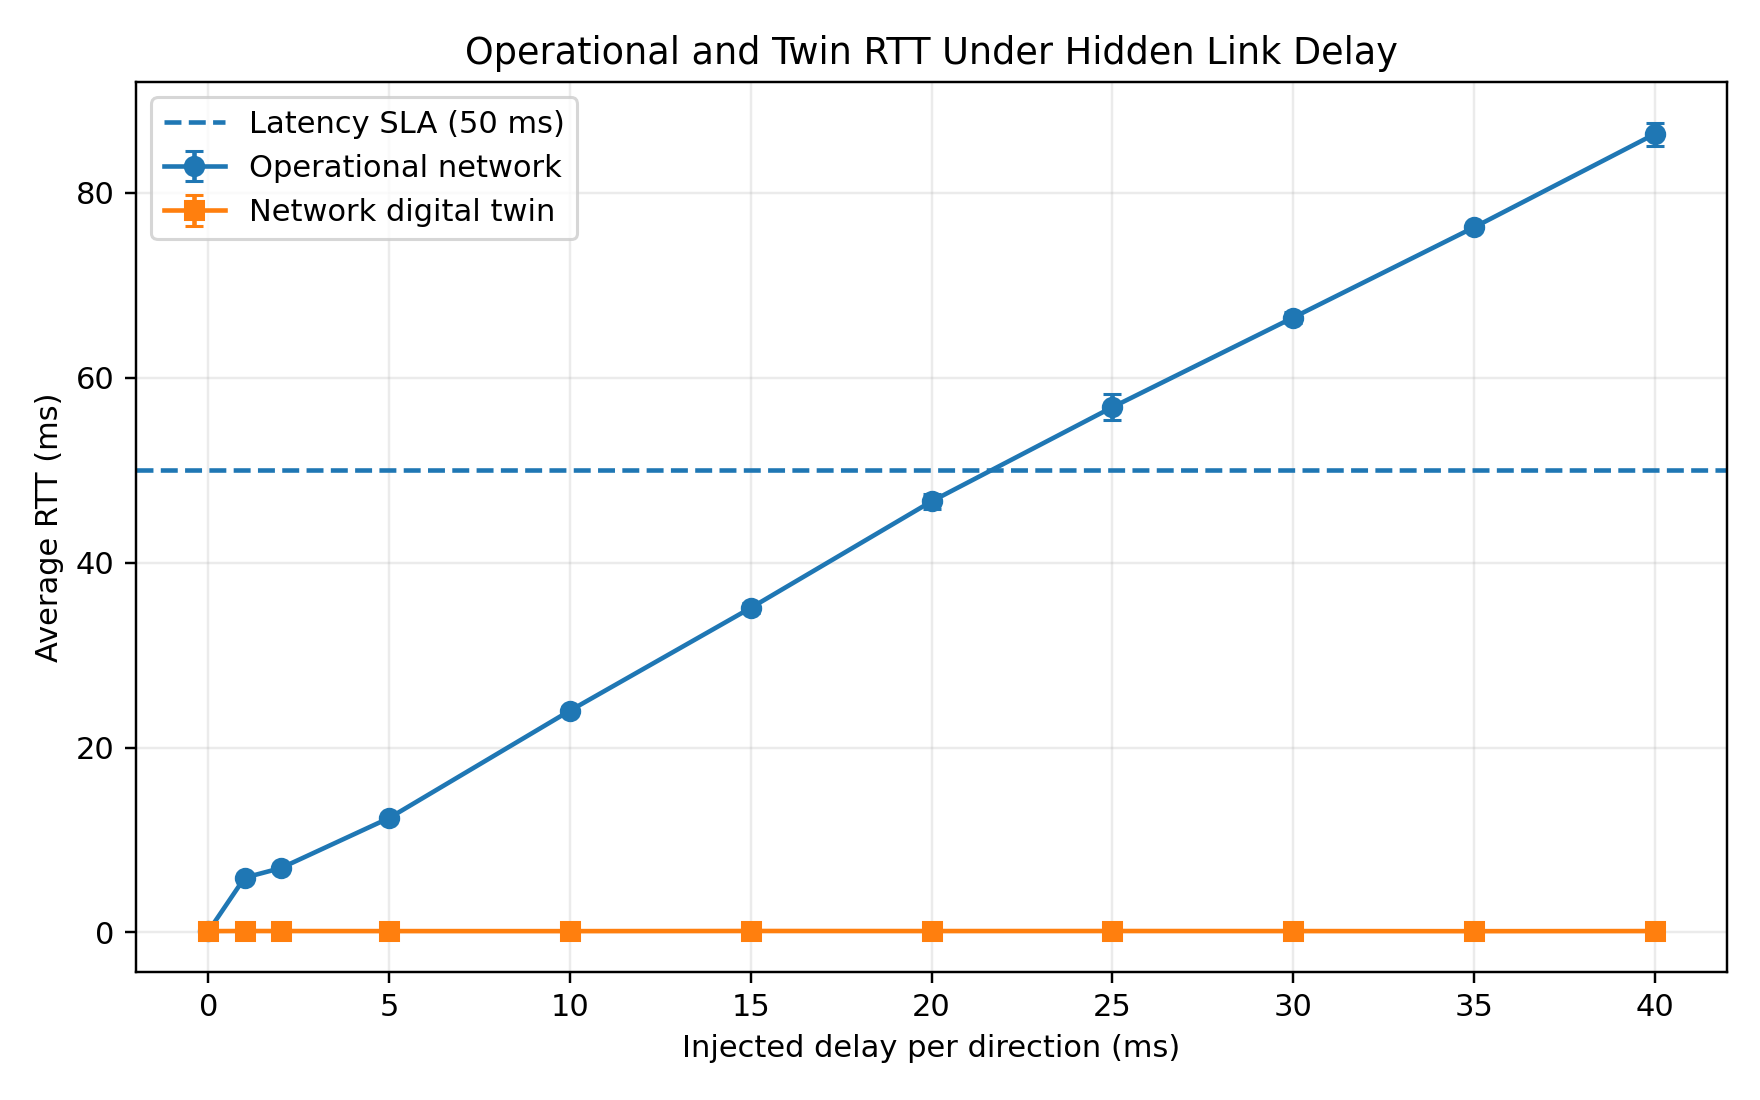
\includegraphics[width=\columnwidth]{figures/figure1_rtt_vs_delay.png}
\caption{Operational and twin RTT as hidden candidate-link delay increases.}\label{fig:rtt-delay}
\end{figure}

\subsection{RQ2: Residual-only gates become unsafe or vacuous}\label{rq2-residual-only-gates-become-unsafe-or-vacuous}

Phase 4 evaluates 186 validation candidates after calibration on 22 samples. Direct deployment, twin-only validation, and a fixed 10 ms margin accept every candidate and each deploys 65 unsafe changes. The static upper residual margin is 85.569 ms, which already exceeds the 50 ms SLA; it therefore rejects all 186 candidates, including all 121 safe candidates.

Rolling residual calibration does not provide a satisfactory compromise. Window 10 accepts only 16 candidates, admits two unsafe changes, and covers 14 of 121 safe candidates. Its safe coverage is 11.57\%. Windows 20 and 50 accept no candidate. Window 10 also fails to accept a safe candidate in any of the three randomized validation schedules.

\begin{table*}[t]
\caption{Residual-only policy outcomes on the Phase 4 validation set.}
\centering
\scriptsize
\begin{tabularx}{\textwidth}{XXXXXX}
\toprule
Policy & Accepted & Unsafe deployed & Safe accepted & Safe coverage & Interpretation \\
\midrule
Direct & 186 & 65 & 121 & 100.00\% & Unsafe baseline \\
Twin only & 186 & 65 & 121 & 100.00\% & Twin fails to detect hidden drift \\
Static residual quantile & 0 & 0 & 0 & 0.00\% & Complete abstention \\
Rolling residual, window 10 & 16 & 2 & 14 & 11.57\% & Low utility and incomplete safety \\
Rolling residual, window 20 & 0 & 0 & 0 & 0.00\% & Complete abstention \\
Rolling residual, window 50 & 0 & 0 & 0 & 0.00\% & Complete abstention \\
\bottomrule
\end{tabularx}
\end{table*}

These results support the negative conclusion that a global residual history does not provide robust operational utility in the tested mixture of latency regimes. Zero unsafe deployments under complete abstention is not treated as a successful safety result.

\begin{figure}
\centering

\includegraphics[width=\columnwidth]{figures/figure3_policy_tradeoff.png}
\caption{Trade-off among residual-only policies.}\label{fig:residual-tradeoff}
\end{figure}

\subsection{RQ3: Candidate-link sensing restores useful discrimination}\label{rq3-candidate-link-sensing-restores-useful-discrimination}

Phase 5 uses the same 22 calibration observations and 186 validation observations, but augments the twin prediction with the operational/twin RTT difference measured on the candidate link. The validation partition contains 112 safe and 74 unsafe candidates.

Direct and twin-only deployment accept every candidate and deploy all 74 unsafe changes. The raw sentinel accepts 111 candidates: 109 safe and two unsafe. Adding the frozen 0.661 ms margin accepts 110 candidates: 109 safe and one unsafe. Thus, the conformal sentinel reduces unsafe deployments by

\[
\frac{74-1}{74}\times100 = 98.65\%
\]

relative to twin-only validation, while retaining 97.32\% safe-change coverage.

\begin{table*}[t]
\caption{Candidate-link policy outcomes on the Phase 5 validation set.}
\centering
\scriptsize
\begin{tabularx}{\textwidth}{XXXXXX}
\toprule
Policy & Accepted & Unsafe deployed & Unsafe among accepted & Safe accepted & Safe coverage \\
\midrule
Direct & 186 & 74 & 39.78\% & 112 & 100.00\% \\
Twin only & 186 & 74 & 39.78\% & 112 & 100.00\% \\
Raw candidate-link sentinel & 111 & 2 & 1.80\% & 109 & 97.32\% \\
Conformal candidate-link sentinel & 110 & 1 & 0.91\% & 109 & 97.32\% \\
\bottomrule
\end{tabularx}
\end{table*}

The single unsafe accepted validation candidate occurs at 20 ms per-direction delay. Its corrected prediction is 48.922 ms, its upper score is 49.583 ms, and its observed RTT is 50.229 ms. Three safe candidates are rejected, also around the 20 ms decision boundary. This concentration indicates that remaining classification error is associated with measurement variation near the SLA rather than failure to detect high-delay regimes.

Across validation, the link correction reduces mean absolute prediction error from 38.154 ms to 0.745 ms. The corrected prediction has Pearson correlation \(r=0.9993\) with observed RTT.

\begin{figure}
\centering
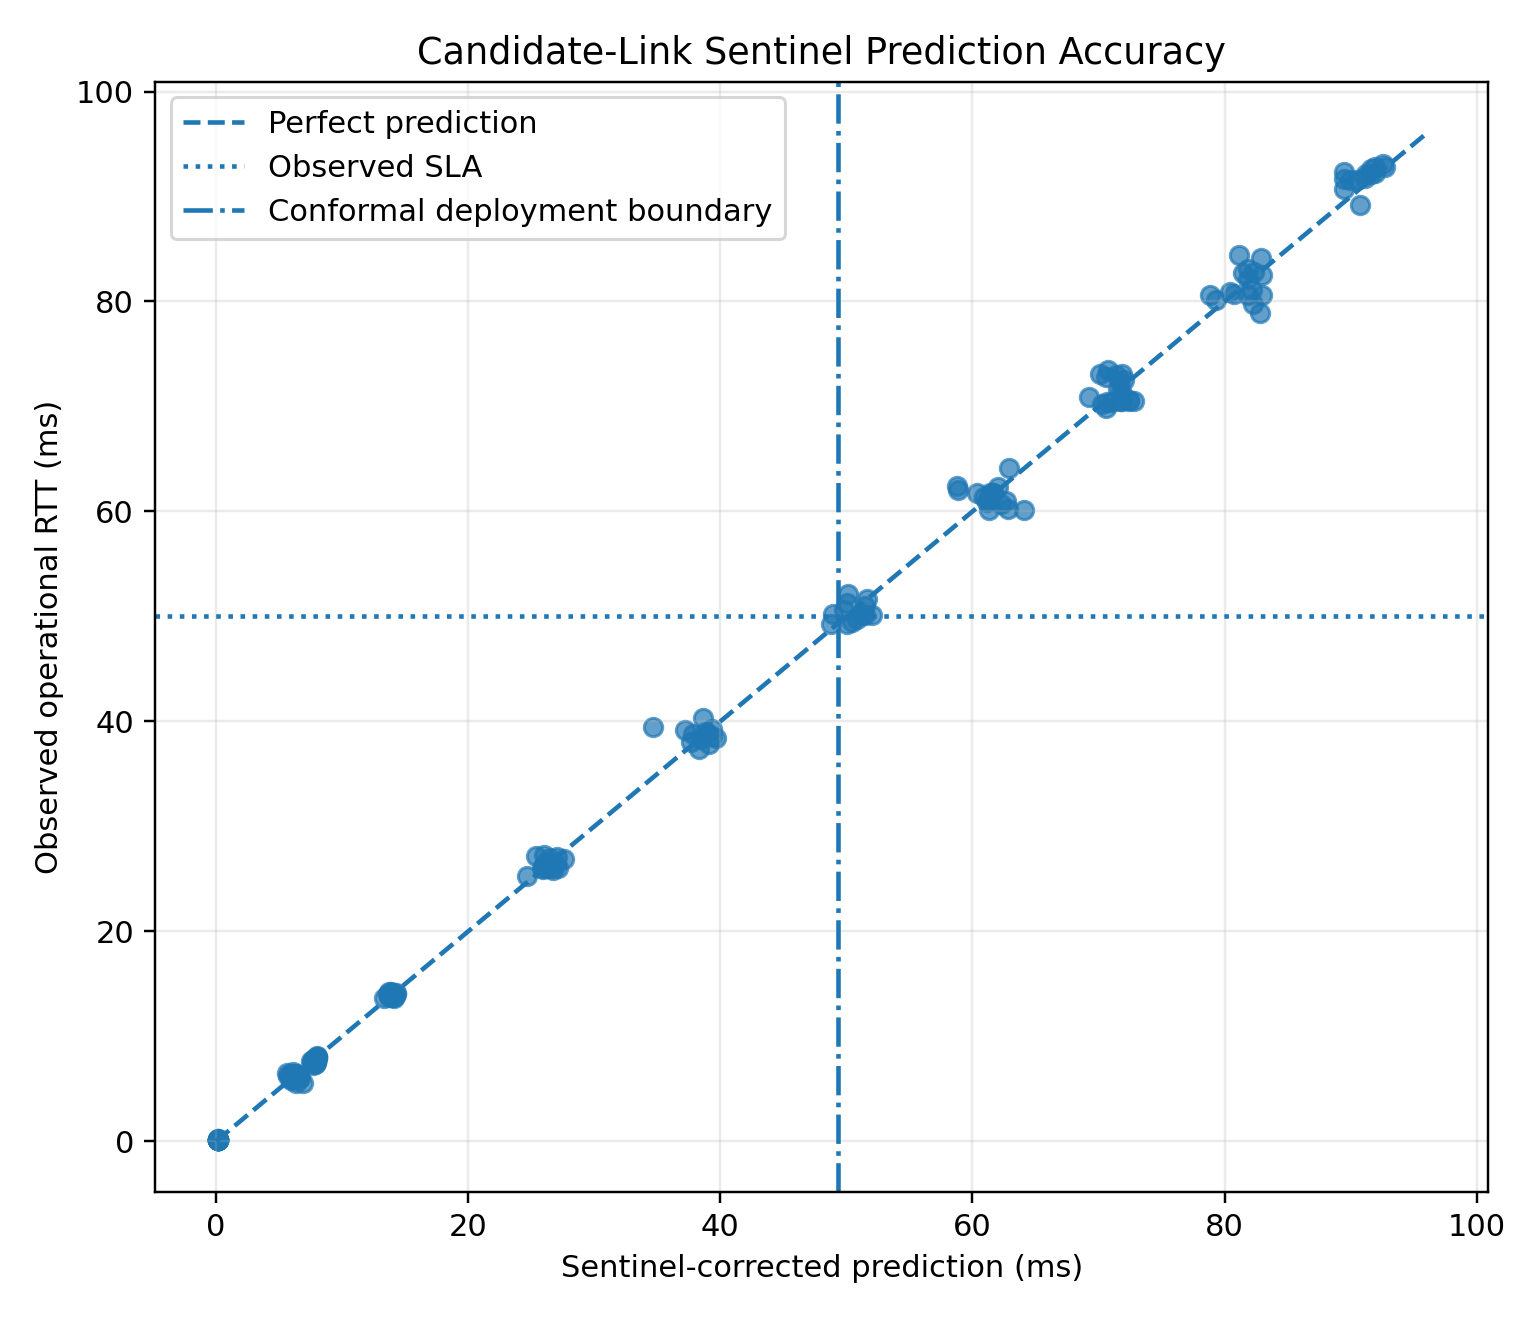
\includegraphics[width=\columnwidth]{figures/phase5_prediction_vs_observed.png}
\caption{Corrected prediction against observed operational RTT during validation.}\label{fig:validation-prediction}
\end{figure}

\subsection{RQ4: The frozen policy retains correct decisions on the untouched holdout}\label{rq4-the-frozen-policy-generalizes-on-the-untouched-holdout}

The frozen conformal sentinel is evaluated once on the 33-sample \texttt{holdout\_seed909} schedule. The holdout contains 19 safe candidates and 14 unsafe candidates. The policy accepts all 19 safe candidates, rejects all 14 unsafe candidates, and makes no observed false-safe or false-reject decision.

\begin{table*}[t]
\caption{Confusion matrix for the untouched holdout.}
\centering
\scriptsize
\begin{tabularx}{\textwidth}{XXX}
\toprule
Actual outcome & Deploy & Reject \\
\midrule
Safe & 19 & 0 \\
Unsafe & 0 & 14 \\
\bottomrule
\end{tabularx}
\end{table*}

The holdout acceptance rate is 57.58\%, close to the 59.14\% validation acceptance rate. No unsafe deployment is observed among the 19 accepted changes. The 95\% Wilson interval for the unsafe rate among accepted changes is 0.00\%--16.82\%, so the experiment does not establish zero underlying risk. The 95\% Wilson interval for the 33/33 observed decision accuracy is 89.57\%--100.00\%.

The raw sentinel would have accepted one additional holdout candidate. For that case, the corrected prediction is 49.985 ms, the frozen upper score is 50.646 ms, and the realized RTT is 50.967 ms. The 0.661 ms margin therefore prevents one unsafe deployment without rejecting a safe holdout candidate.

\begin{figure}
\centering
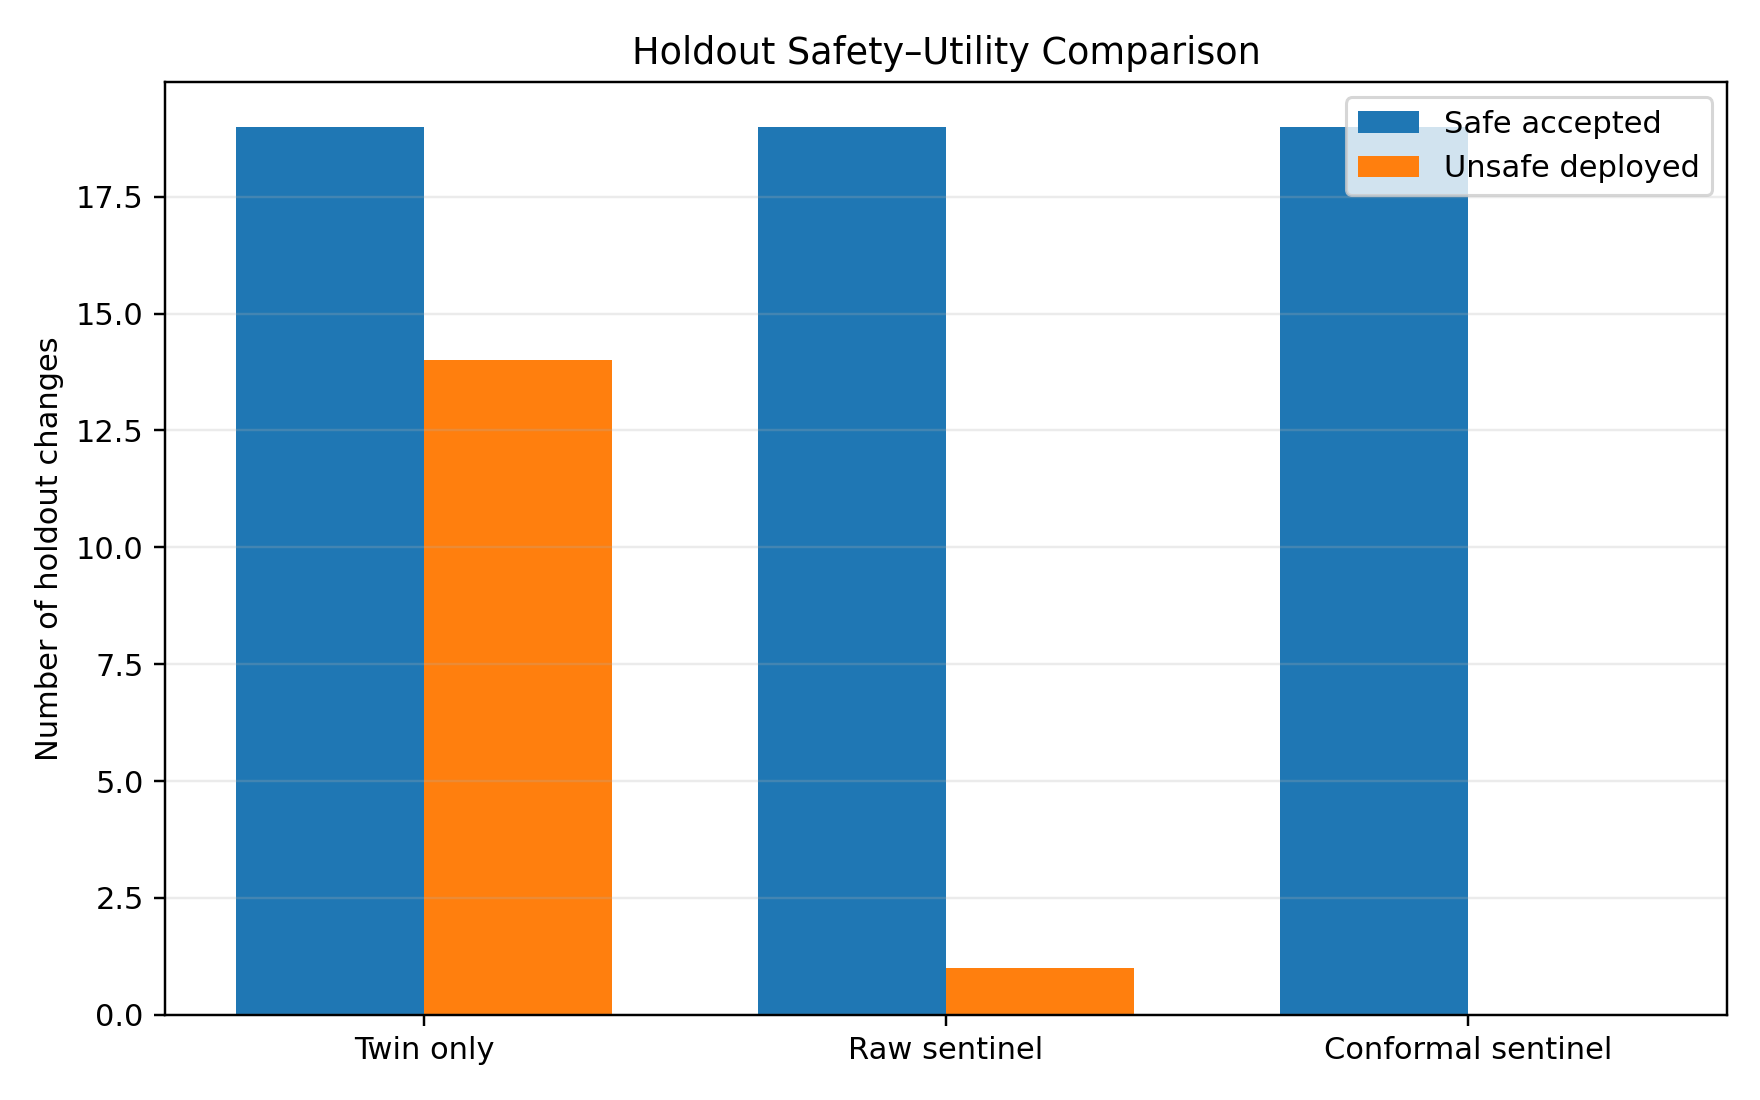
\includegraphics[width=\columnwidth]{figures/phase5_holdout_policy_comparison.png}
\caption{Safety and utility of the holdout policies.}\label{fig:holdout-policy}
\end{figure}

\subsection{Prediction accuracy and conformal-bound coverage are different outcomes}\label{prediction-accuracy-and-conformal-bound-coverage-are-different-outcomes}

The candidate-link correction remains accurate on the holdout: mean absolute error falls from 40.917 ms for the uncorrected twin to 0.990 ms, with Pearson correlation \(r=0.9991\).

\begin{table*}[t]
\caption{Prediction accuracy and empirical upper-bound coverage.}
\centering
\scriptsize
\begin{tabularx}{\textwidth}{XXXXXXX}
\toprule
Partition & Samples & Twin-only MAE (ms) & Corrected MAE (ms) & Corrected RMSE (ms) & Pearson r & Upper-bound coverage \\
\midrule
Validation & 186 & 38.154 & 0.745 & 1.149 & 0.9993 & 150/186 (80.65\%) \\
Holdout & 33 & 40.917 & 0.990 & 1.440 & 0.9991 & 20/33 (60.61\%) \\
\bottomrule
\end{tabularx}
\end{table*}

However, the one-sided upper score covers only 150/186 validation observations (80.65\%) and 20/33 holdout observations (60.61\%). Nominal 95\% predictive coverage therefore does not persist under the shifted residual distribution.

The empirical deployment classifier and the predictive interval must not be conflated. The classifier performs strongly because safe and unsafe candidates are separated around the fixed 50 ms decision boundary in this experiment. The interval itself does not satisfy the nominal coverage target. The result supports empirical deployment safety and utility in the tested setting, not a distribution-free conformal guarantee.

\begin{figure}
\centering
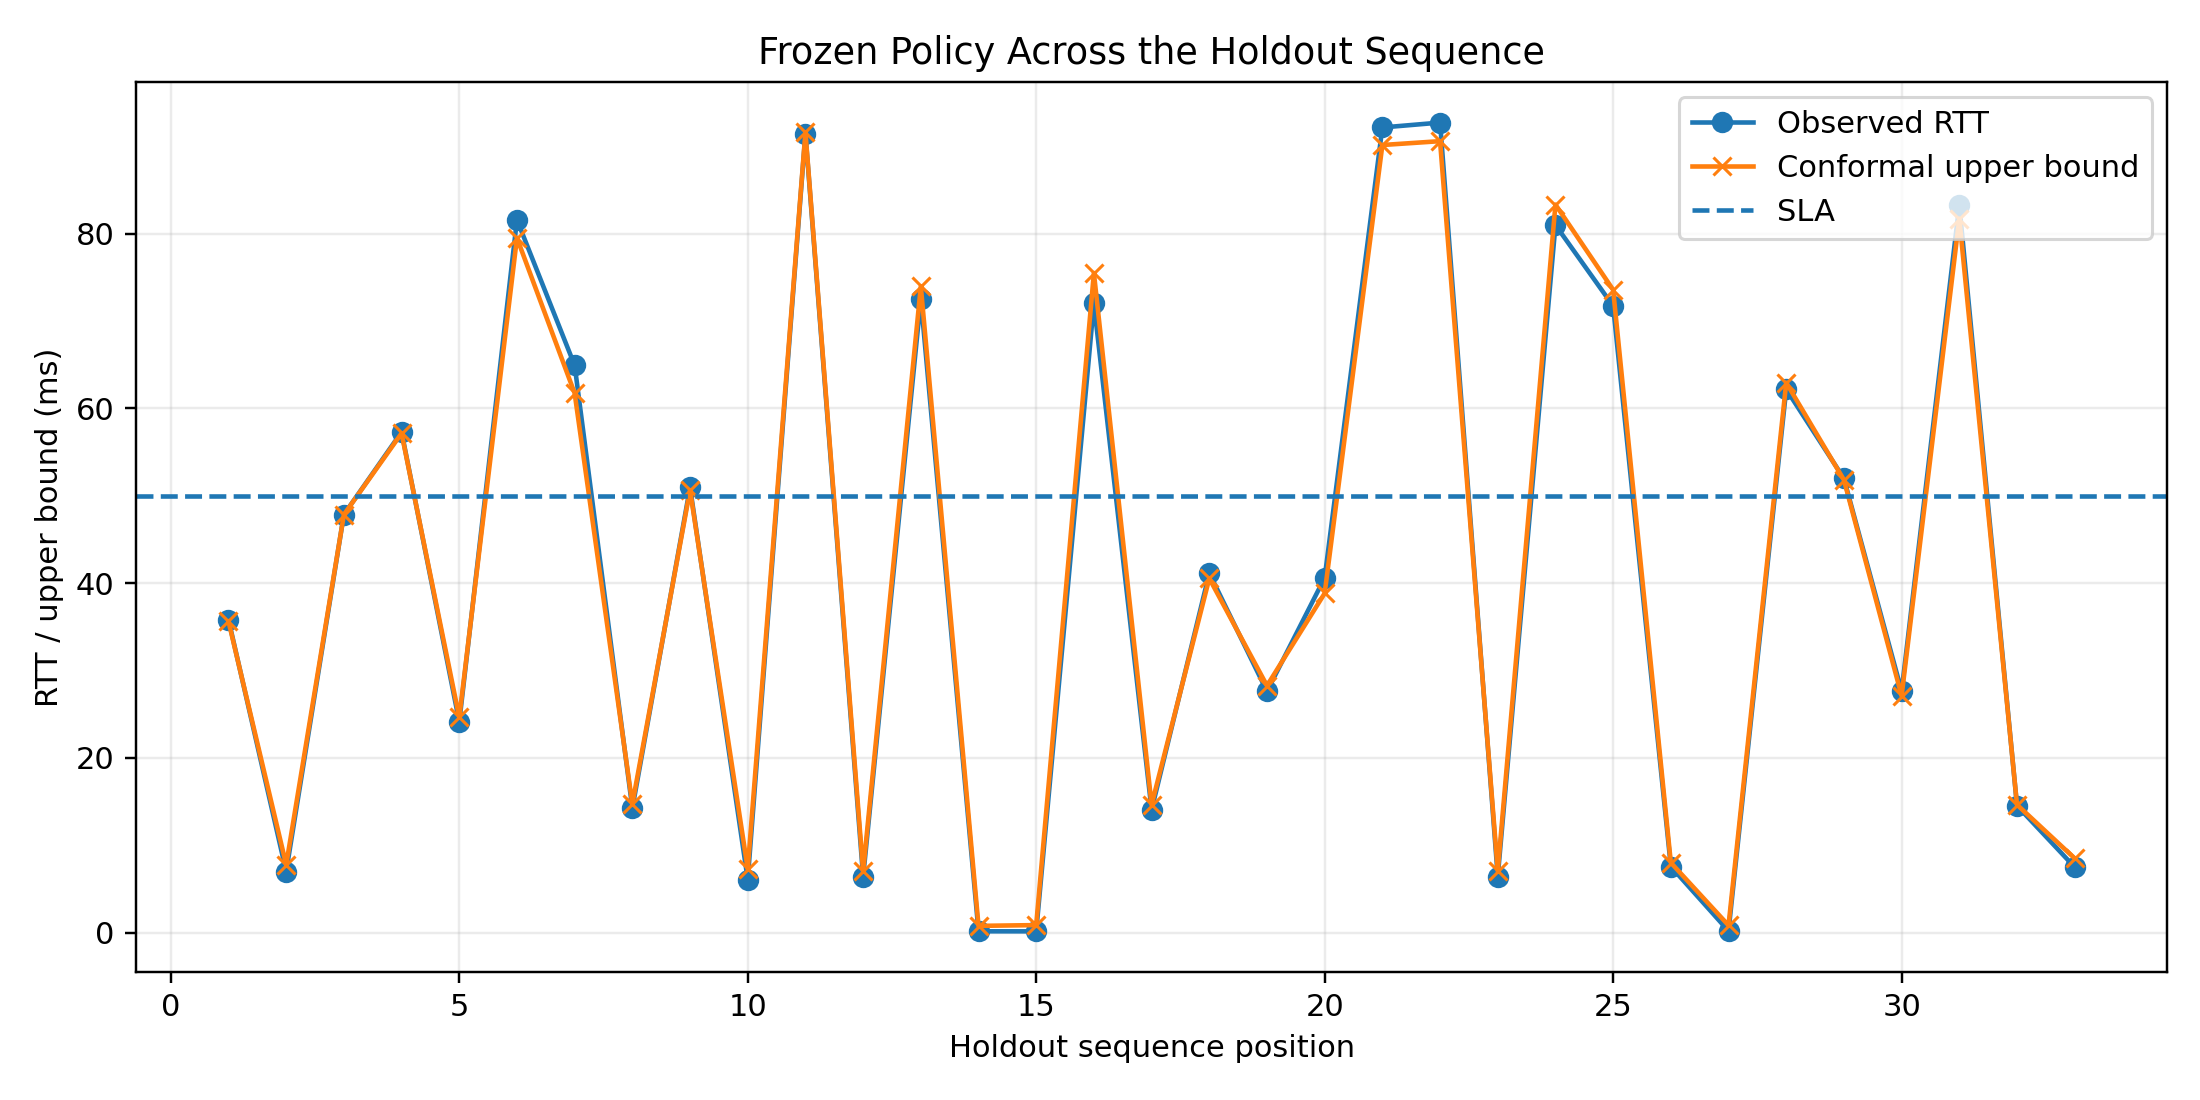
\includegraphics[width=\columnwidth]{figures/phase5_holdout_sequence.png}
\caption{Frozen upper score and observed RTT through the holdout sequence.}\label{fig:holdout-sequence}
\end{figure}

\subsection{Summary of research questions}\label{summary-of-research-questions}

\begin{itemize}
\tightlist
\item
  \textbf{RQ1:} Yes. Route agreement does not prevent a false-safe latency decision when the activated operational link has hidden delay.
\item
  \textbf{RQ2:} No residual-only policy tested provides both robust safety and useful acceptance; several collapse into complete abstention.
\item
  \textbf{RQ3:} Yes. Candidate-link correction sharply reduces prediction error and unsafe deployments while retaining high safe coverage.
\item
  \textbf{RQ4:} Yes within the tested schedule. The frozen policy makes no observed classification error on the 33-sample holdout, but the sample is small and nominal conformal coverage fails.
\end{itemize}

\section{Discussion}\label{discussion}

\subsection{Why the targeted sentinel works}\label{why-the-targeted-sentinel-works}

The false-safe failure is caused by a localized mismatch: the candidate OSPF change activates a direct link whose operational delay is absent from the twin. A global historical residual does not identify where the mismatch lies and can mix observations from substantially different delay regimes. The candidate-link sentinel instead measures the component most likely to determine the post-change path.

In this controlled topology, the operational/twin link RTT difference transfers directly to the end-to-end candidate path. The correction therefore removes most of the dominant error while requiring only a small pre-deployment probe. This is an example of using configuration semantics to choose a high-value measurement: the proposed OSPF change identifies the link that requires additional validation.

\subsection{Safety, utility, and abstention}\label{safety-utility-and-abstention}

A deploy/reject policy cannot be assessed by unsafe deployments alone. Rejecting every candidate trivially produces zero deployed failures but prevents all beneficial changes. Phase 4 demonstrates this problem directly: the static margin and rolling windows of 20 and 50 observations abstain completely, whereas the 10-observation window trades that vacuity for two unsafe deployments and inconsistent cross-schedule utility.

The candidate-link sentinel provides a more useful balance. It rejects high delay candidates while accepting nearly all safe validation candidates and all safe holdout candidates. The policy-selection rule formalizes this by requiring safe acceptance in every validation schedule before minimizing unsafe deployments.

\subsection{The role of the conformal margin}\label{the-role-of-the-conformal-margin}

The raw sentinel performs most of the correction. The frozen margin is small relative to the hidden delay and changes only candidates close to the SLA. It removes one unsafe validation decision and one unsafe holdout decision that the raw sentinel would accept, while preserving the same validation safe coverage and all holdout safe candidates.

This result does not validate the margin as a nominal 95\% prediction bound. Its empirical value here is decision-boundary protection. A future method should calibrate explicitly for decision risk under nonstationarity rather than interpreting a static split-conformal quantile as valid after arbitrary distribution shift.

\subsection{Implications for NDT-assisted automation}\label{implications-for-ndt-assisted-automation}

The experiment suggests a general control pattern:

\begin{enumerate}
\def\labelenumi{\arabic{enumi}.}
\tightlist
\item
  use the candidate configuration to predict which resources or links will become critical;
\item
  obtain targeted operational measurements of those resources before deployment;
\item
  compare them with their twin representations;
\item
  correct or invalidate the twin's prediction; and
\item
  abstain when the corrected upper score violates policy.
\end{enumerate}

An agent-generated change could invoke this validator before execution. Formal configuration verification would still be used to check reachability, loops, and protocol behavior; consistent-update mechanisms would still govern installation. The sentinel adds a complementary performance-fidelity check.

\subsection{Feedback availability}\label{feedback-availability}

The candidate-link probe is available for rejected candidates, which avoids a key weakness of outcome-only online adaptation: a controller does not need to deploy an unsafe candidate to learn that the relevant link has drifted. The post-change end-to-end outcome is still useful for monitoring and recalibration after accepted deployments.

For more complex candidates, the active resource set may contain several links or nodes. Extending the method would require automatic path differencing, multiple probes, and a rule for combining their discrepancies.

\subsection{Decision accuracy versus interval validity}\label{decision-accuracy-versus-interval-validity}

The holdout illustrates why binary accuracy and predictive coverage should be reported separately. Every holdout decision is correct relative to the 50 ms threshold, yet the upper score covers only 20 of 33 realized RTTs. Favorable separation around the SLA can produce accurate decisions even when residual tails differ from calibration.

The paper therefore avoids describing the method as a conformal guarantee under drift. Weighted conformal prediction, adaptive conformal inference, or risk-controlling prediction sets are plausible extensions, but each requires additional assumptions, feedback, and evaluation.

\section{Limitations and Threats to Validity}\label{limitations-and-threats-to-validity}

\subsection{Topology and protocol scope}\label{topology-and-protocol-scope}

The testbed contains three routers in one OSPF area and evaluates one bidirectional cost change. The candidate link is manually identified. Results cannot be assumed to transfer to multi-area OSPF, equal-cost multipath, multiple simultaneous weight changes, route redistribution, or large production networks.

\subsection{Drift scope}\label{drift-scope}

The manipulated drift is fixed latency applied to one direct link. The study does not evaluate loss, bandwidth reduction, queue buildup, jitter as a primary outcome, failed links, topology drift, asymmetric impairments, multiple drifting resources, or adversarial telemetry.

\subsection{Measurement scope}\label{measurement-scope}

Mean ICMP RTT is the only deployment SLA. It does not represent application response time, tail latency, throughput, or service-specific quality. Twenty probes reduce noise but do not eliminate container scheduling and active measurement variation.

\subsection{Experimental enforcement}\label{experimental-enforcement}

Every candidate is operationally applied in the harness so that rejected candidates receive a ground-truth label. Policy decisions are replayed only from pre-deployment fields, but the artifact is an offline labeled evaluation rather than a live controller that blocks rejected changes.

\subsection{Sample size and schedule support}\label{sample-size-and-schedule-support}

Calibration uses 22 observations and the holdout contains 33 observations. The delay values are discrete and known to the experimental design. Wilson intervals remain wide, and perfect holdout classification should not be interpreted as proof of negligible production risk.

\subsection{Statistical assumptions}\label{statistical-assumptions}

The frozen split-conformal-style margin does not retain nominal 95\% predictive coverage on validation or holdout. Exchangeability under the residual distribution is not established. The study therefore makes no distribution-free coverage or risk-control claim.

\subsection{Procedural deviation}\label{procedural-deviation}

The first holdout measurement was collected before the policy manifest was committed because the results directory was initially ignored by Git. Parsing failed, the raw files were retained, and only the parser was changed to accept the observed BusyBox format. The policy values already existed and were not changed after the measurement. The incident is documented, but it remains a deviation from the ideal sequence in which the manifest commit precedes every holdout observation.

\subsection{Researcher degrees of freedom}\label{researcher-degrees-of-freedom}

The sentinel was introduced after residual-only methods failed in Phase 4. This is legitimate method development, but Phase 4 is exploratory rather than confirmatory evidence for the final method. Confirmatory support comes from the policy-freezing protocol and the separate holdout. Independent replication would provide stronger evidence.

\section{Reproducibility and Artifact Availability}\label{reproducibility-and-artifact-availability}

The artifact contains separate Containerlab definitions for the operational network and twin, FRRouting configurations, generated experiment schedules, measurement and parsing scripts, processed calibration, validation, and holdout datasets, the frozen policy manifest, analysis outputs, figures, and dated provenance records for the experimental milestones.

Key reproducibility records include:

\begin{itemize}
\tightlist
\item
  \path{lab/phase5/results/frozen_policy.json};
\item
  \path{lab/phase5/results/validation_results.json};
\item
  \path{lab/phase5/results/holdout_results.json};
\item
  \path{processed-data/phase5_sentinel_dataset.csv};
\item
  \path{processed-data/phase5_holdout_dataset.csv};
\item
  \path{docs/holdout_execution_log.md};
\item
  \path{docs/phase5_evaluator_correction.md}; and
\item
  \path{docs/method_implementation_traceability.csv}.
\end{itemize}

The frozen manifest records SHA-256 hashes for the dataset and the historical pre-correction validation artifacts. The latter are preserved with \texttt{\_original} suffixes, and \texttt{frozen\_hash\_resolution.json} records the filename mapping without changing the frozen manifest. Holdout outputs have a separate hash list. The holdout runner refuses automatic re-evaluation after the final results file exists. Corrected validation outputs and later recomputations use distinct filenames so that the historical decision artifacts remain intact.

A versioned release archive, \texttt{ndt-ospf-artifact-v1.0.0.zip}, has been prepared with the code, configurations, processed data, frozen manifests, analysis outputs, figures, and checksums. A permanent public URL and DOI will be added in a subsequent arXiv version after repository and Zenodo deposit.

\section{Conclusion}\label{conclusion}

A network digital twin can agree with an operational network on OSPF convergence, route metric, and next hop while still approving a change that violates an operational latency SLA. In the controlled experiment, this false-safe behavior is caused by hidden delay on the direct link activated by the candidate cost change.

Residual-only uncertainty gates do not solve the problem reliably: the tested static and larger rolling margins collapse into complete abstention, while the smaller rolling window remains unsafe. A targeted candidate-link probe provides a more useful signal. By correcting the twin prediction with the operational/twin link discrepancy and applying a frozen 0.661 ms margin, the selected policy reduces unsafe validation deployments from 74 to one while retaining 97.32\% safe coverage. On the 33-sample untouched holdout, it accepts all 19 safe candidates and rejects all 14 unsafe candidates.

The result is an empirical demonstration, not a universal safety guarantee. Nominal conformal predictive coverage fails under the shifted residual distribution, and the topology, drift model, and sample size are limited. Nevertheless, the study identifies a concrete design principle for safer NDT-assisted automation: use the semantics of a proposed network change to measure the resources it will activate before trusting the twin's performance prediction.




\section*{Declarations}
\textit{Funding:} This research received no external funding.
\textit{Competing interests:} The author declares no competing interests.

\section{Data and Code Availability}
The release \texttt{ndt-ospf-artifact-v1.0.0.zip} contains the Containerlab
and FRRouting configurations, schedules, measurement and analysis code,
processed calibration, validation, and holdout data, the frozen policy,
figures, and SHA-256 checksums. The holdout is archival evidence and must not
be reused for tuning. A permanent repository URL and Zenodo DOI will be added
after public deposit.

\section*{Author Contributions}
The author conceived the study, implemented the testbed, conducted the
experiments, analyzed the data, and prepared the manuscript and reproducibility
artifact.

\begin{thebibliography}{99}
\bibitem{zhou2026ndtarch} C. Zhou \emph{et al.}, {``Network digital twin ({NDT}): Concepts and reference architecture,''} Internet Research Task Force, draft-irtf-nmrg-network-digital-twin-arch-13, Jul. 2026.

\bibitem{zhou2026datacollection} C. Zhou, D. Chen, P. Martinez-Julia, and Q. Ma, {``Data collection requirements and technologies for network digital twin,''} Internet Engineering Task Force, draft-zcz-nmrg-digitaltwin-data-collection-05, Jul. 2026.

\bibitem{moy1998ospf} J. Moy, {``{OSPF Version 2},''} RFC Editor, RFC 2328, Apr. 1998. doi: \href{https://doi.org/10.17487/RFC2328}{10.17487/RFC2328}.

\bibitem{fortz2000ospf} B. Fortz and M. Thorup, {``Internet traffic engineering by optimizing {OSPF} weights,''} in \emph{Proceedings IEEE INFOCOM 2000}, 2000, pp. 519--528. doi: \href{https://doi.org/10.1109/INFCOM.2000.832225}{10.1109/INFCOM.2000.832225}.

\bibitem{fogel2015batfish} A. Fogel \emph{et al.}, {``A general approach to network configuration analysis,''} in \emph{12th USENIX symposium on networked systems design and implementation (NSDI 15)}, 2015, pp. 469--483.

\bibitem{beckett2017minesweeper} R. Beckett, A. Gupta, R. Mahajan, and D. Walker, {``A general approach to network configuration verification,''} in \emph{Proceedings of the 2017 ACM SIGCOMM conference}, 2017, pp. 155--168.

\bibitem{prabhu2020plankton} S. Prabhu, K.-Y. Chou, A. Kheradmand, P. B. Godfrey, and M. Caesar, {``Plankton: Scalable network configuration verification through model checking,''} in \emph{17th USENIX symposium on networked systems design and implementation (NSDI 20)}, 2020, pp. 953--967.

\bibitem{reitblatt2012updates} M. Reitblatt, N. Foster, J. Rexford, C. Schlesinger, and D. Walker, {``Abstractions for network update,''} in \emph{Proceedings of the ACM SIGCOMM 2012 conference}, 2012, pp. 323--334. doi: \href{https://doi.org/10.1145/2342356.2342427}{10.1145/2342356.2342427}.

\bibitem{tibshirani2019covariate} R. J. Tibshirani, R. F. Barber, E. J. Candès, and A. Ramdas, {``Conformal prediction under covariate shift,''} \emph{arXiv preprint arXiv:1904.06019}, 2019, doi: \href{https://doi.org/10.48550/arXiv.1904.06019}{10.48550/arXiv.1904.06019}.

\bibitem{gibbs2021adaptive} I. Gibbs and E. Candès, {``Adaptive conformal inference under distribution shift,''} in \emph{Advances in Neural Information Processing Systems}, vol. 34, pp. 1660--1672, 2021.

\bibitem{gibbs2024online} I. Gibbs and E. J. Candès, {``Conformal inference for online prediction with arbitrary distribution shifts,''} \emph{Journal of Machine Learning Research}, vol. 25, no. 162, pp. 1--36, 2024.

\bibitem{almasan2022ndt} P. Almasan \emph{et al.}, {``Network digital twin: Context, enabling technologies and opportunities,''} \emph{IEEE Communications Magazine}, 2022, doi: \href{https://doi.org/10.1109/MCOM.001.2200012}{10.1109/MCOM.001.2200012}.

\bibitem{hui2022performance} L. Hui, M. Wang, L. Zhang, L. Lu, and Y. Cui, {``Digital twin for networking: A data-driven performance modeling perspective,''} \emph{arXiv preprint arXiv:2206.00310}, 2022, doi: \href{https://doi.org/10.48550/arXiv.2206.00310}{10.48550/arXiv.2206.00310}.

\bibitem{abenathar2025routeopt} R. Aben-Athar \emph{et al.}, {``Network digital twin for route optimization in 5G/B5G transport slicing with what-if analysis,''} \emph{arXiv preprint arXiv:2505.04879}, 2025, doi: \href{https://doi.org/10.48550/arXiv.2505.04879}{10.48550/arXiv.2505.04879}.

\bibitem{auge2026aether} J. Auge, S. Betts, G. Carofiglio, G. Grassi, M. Gysi, and J. K. d'Souza, {``Aether: Network validation using agentic AI and digital twin,''} \emph{arXiv preprint arXiv:2604.18233}, 2026, doi: \href{https://doi.org/10.48550/arXiv.2604.18233}{10.48550/arXiv.2604.18233}.

\bibitem{miao2026mirrornet} C. Miao \emph{et al.}, {``MirrorNet: High-fidelity and scalable network emulation for software-defined WAN,''} in \emph{23rd USENIX Symposium on Networked Systems Design and Implementation (NSDI 26)}, USENIX Association, May 2026, pp. 175--190.

\bibitem{xia2026real} Z. Xia, H. Li, J. Fu, X. Wan, Y. Dang, D. Shan, L. Chen, and P. Zhang, {``REAL: Emulating control plane at simulator's cost,''} in \emph{23rd USENIX Symposium on Networked Systems Design and Implementation (NSDI 26)}, USENIX Association, May 2026, pp. 1861--1877.

\bibitem{wu2026agentndt} Q. Wu, C. Zhou, L. M. Contreras, S. Han, and Y.-G. Hong, {``Network digital twin and agentic AI based architecture for AI driven network operations,''} Internet Engineering Task Force, draft-wmz-nmrg-agent-ndt-arch-04, May 2026.

\bibitem{bates2021risk} S. Bates, A. Angelopoulos, L. Lei, J. Malik, and M. I. Jordan, {``Distribution-free, risk-controlling prediction sets,''} \emph{Journal of the ACM}, vol. 68, no. 6, 2021, doi: \href{https://doi.org/10.1145/3478535}{10.1145/3478535}.

\end{thebibliography}

\end{document}
